\documentclass[14pt]{extarticle}
\usepackage[english,ukrainian]{babel}
\usepackage[utf8]{inputenc}
\usepackage{amsmath,amssymb}
\usepackage{parskip}
\usepackage{graphicx}
\usepackage{xcolor}
\usepackage{tcolorbox}
\tcbuselibrary{skins}
\usepackage[framemethod=tikz]{mdframed}
\usepackage{chngcntr}
\usepackage{enumitem}
\usepackage{hyperref}
\usepackage{float}
\usepackage{subfig}
\usepackage{esint}
\usepackage[top=2.5cm, left=3cm, right=3cm, bottom=4.0cm]{geometry}
\usepackage[table]{xcolor}
\usepackage{algorithm}
\usepackage{algpseudocode}
\usepackage{listings}
\usepackage{xcolor}

\title{Домашня робота \#2 (друга частина) з курсу ``Комплексний аналіз''}
\author{Студента 3 курсу групи МП-31 Захарова Дмитра}
\date{\today}

\begin{document}

\maketitle

\section*{Завдання 1 (Тест 7.1 \#4).}

\textbf{Умова.} Обчислити інтеграл:
\[
\int_{\mathcal{C}} (2x-iy)dz, \; \mathcal{C} = \{z \in \mathbb{C}: |z| = 1 \wedge \text{Re}\, z > 0\}
\]

\textbf{Розв'язок.} Помітимо, що $dz=dx+idy$, тому
\[
\mathcal{I} := \int_{\mathcal{C}} (2x-iy)(dx+idy) = \int_{\mathcal{C}}(2x - iy)dx + \int_{\mathcal{C}} (2ix + y)dy
\]
Або можемо розбити на чотири інтеграли:
\[
\mathcal{I} = 2\int_{\mathcal{C}}xdx - i\int_{\mathcal{C}}ydx + 2i\int_{\mathcal{C}}xdy + \int_{\mathcal{C}} ydy
\]

Тепер треба параметризувати $\mathcal{C}$. Коло параметризується $z(\varphi) = e^{i\varphi}$, проте треба обрати межу. Оскільки маємо праве півколо, то межі $\varphi \in \left[-\frac{\pi}{2},\frac{\pi}{2}\right]$. Тоді $x=\cos\varphi, y = \sin\varphi, dz=ie^{i\varphi}d\varphi$, тому $dx=\text{Re} \, dz=-\sin\varphi d\varphi, dy=\text{Im}\, dz = \cos\varphi d\varphi$. Тому можемо знайти кожен з інтегралів.

\textit{Перший інтеграл ($2\int_{\mathcal{C}}xdx$).}
\[
2\int_{\mathcal{C}} xdx = -2\int_{-\pi/2}^{\pi/2}\cos\varphi\sin\varphi d\varphi = -\int_{-\pi/2}^{\pi/2} \sin 2\varphi d\varphi = \frac{\cos \pi - \cos(-\pi)}{2} = 0
\]
\textit{Другий інтеграл ($i\int_{\mathcal{C}}ydx$).}
\begin{align*}
i\int_{\mathcal{C}}ydx = -i\int_{-\pi/2}^{\pi/2}\sin^2\varphi d\varphi = -i \int_{-\pi/2}^{\pi/2} \frac{1-\cos 2\varphi}{2}d\varphi \\ = -\frac{i\pi}{2} + \frac{i}{2}\int_{-\pi/2}^{\pi/2}\cos 2\varphi d\varphi = -\frac{i\pi}{2} + \frac{i(\sin \pi - \sin(-\pi))}{4} = -\frac{i\pi}{2}
\end{align*}
\textit{Третій інтеграл ($2i\int_{\mathcal{C}}xdy$).}
\[
2i\int_{\mathcal{C}}xdy = 2i \int_{-\pi/2}^{\pi/2} \cos^2\varphi d\varphi = 2i \int_{-\pi/2}^{\pi/2} \frac{1+\cos 2\varphi}{2}d\varphi = i\pi + i \int_{-\pi/2}^{\pi/2}\cos 2 \varphi d\varphi = i\pi
\]
\textit{Четвертий інтеграл ($\int_{\mathcal{C}} ydy$).}
\[
\int_{\mathcal{C}}ydy = \int_{-\pi/2}^{\pi/2} \sin\varphi \cos\varphi d\varphi = 0
\]

Отже, по-ітогу:
\[
\mathcal{I} = 0 + \frac{i\pi}{2} + i\pi = \frac{3i\pi}{2}
\]

\textbf{Відповідь.} $\frac{3i\pi}{2}$.

\section*{Завдання 2 (Тест 7.1 \#9).}

\textbf{Умова.} Обчислити інтеграл $\int_{|z-2|=3}(z^2-z)dz$

\textbf{Розв'язок.} 

\textbf{Спосіб I.} Криву $|z-2|=3$ можна параметризувати як $z = 2 + 3e^{i\varphi}$ для $\varphi \in [0,2\pi]$. Тому:
\[
\mathcal{I}=\int_{|z-2|=3}(z^2-z)dz = \int_0^{2\pi} ((2+3e^{i\varphi})^2 - 2 - 3e^{i\varphi})3ie^{i\varphi}d\varphi
\]
Далі спрощуємо:
\begin{gather*}
\mathcal{I} = 3i\int_0^{2\pi}(4+12e^{i\varphi}+9e^{2i\varphi} - 2 - 3e^{i\varphi})e^{i\varphi}d\varphi = \\
3i\int_0^{2\pi} (2e^{i\varphi} + 9e^{2i\varphi} + 9e^{3i\varphi})d\varphi = 6i\int_0^{2\pi}e^{i\varphi}d\varphi + 27i\int_0^{2\pi}e^{2i\varphi}d\varphi + 27i\int_0^{2\pi}e^{3i\varphi}d\varphi
\end{gather*}

Бачимо інтеграли виду $\int_0^{2\pi}e^{i k\varphi}d\varphi$. Проінтегруємо:
\[
\int_0^{2\pi} e^{ik\varphi}d\varphi = \frac{1}{ik} e^{ik\varphi}\Big|_{\varphi=0}^{\varphi=2\pi} = \frac{i(1 - e^{2\pi ki})}{k} = 0
\]
Отже, $\mathcal{I} = 0$. 

\textbf{Спосіб II.} Оскільки функція $f(z)=z^2-z$ голоморфна всередині шара $\mathcal{D}:|z-2|<3$, то згідно теоремі Коші-Гурса $\int_{\partial\mathcal{D}}f(z)dz=0$. 

\section*{Завдання 3 (Тест 8.1 \#7).}
\textbf{Умова.} За допомогою інтегральної формули Коші обчислити інтеграл 
\[
\int_{|z+2|=3} \frac{\sin z}{z+3}dz
\]

\textbf{Розв'язок.} Розглянемо функцію $f(z)=\sin z$. Вона є голоморфною на всьому $\mathbb{C}$, тому за інтегральною формулою Коші:
\[
f(z) = \frac{1}{2\pi i}\int_{\partial\mathcal{D}} \frac{f(\xi)}{\xi - z}d\xi
\]
В нашому випадку:
\[
f(-3) = \frac{1}{2\pi i}\int_{|z+2|=3} \frac{\sin \xi d\xi}{\xi+3} \implies \int_{|z+2|=3} \frac{\sin zdz}{z+3} = 2\pi i \sin(-3)
\]

\textbf{Відповідь.} $2\pi i \sin(-3)$. 

\section*{Завдання 4 (Тест 8.1 \#8)}
\textbf{Умова.} Обрати правильну формулу для обчислення інтеграла $\int_{|z+1|=3}\frac{\sin z}{(z+3)^2}dz$.

\textbf{Розв'язок.} Скористаємося наслідком інтегральної формули Коші:
\[
f^{(n)}(z) = \frac{n!}{2\pi i}\int_{\partial\mathcal{D}} \frac{f(\xi)d\xi}{(\xi - z)^{n+1}}
\]
Отже, розглядаємо $f(z) = \sin z$. Похідна $f'(z)=\cos z$, тому:
\[
f'(-3) = \frac{1}{2\pi i}\int_{|z+1|=3} \frac{\sin z dz}{(z+3)^2} \implies \frac{1}{2\pi i}\int_{|z+1|=3} \frac{\sin z dz}{(z+3)^2} = 2\pi i \cos (-3)
\]
\textbf{Відповідь.} $2\pi i \cos(-3)$.

\section*{Завдання 5 (Тест 8.1 \#9)}
\textbf{Умова.} За допомогою інтегральної формули Коші обчисліть інтеграл
\[
\mathcal{I} = \int_{|z|=2} \frac{dz}{(z-1)(z+1)(z-3)}
\]
\textbf{Розв'язок.} Розіб'ємо коло $|z|=2$ на дві частини: півкулю, де $\text{Re}\, z > 0$ і навпаки. Контур по правій півкулі назвемо $\mathcal{C}_1$, другу півкулю $\mathcal{C}_2$, а лінію по діаметру, відраховуючи зверху, $\mathcal{C}_3$ (див. рис. \ref{fig:2_2_5}).
\begin{figure}[H]
    \centering
    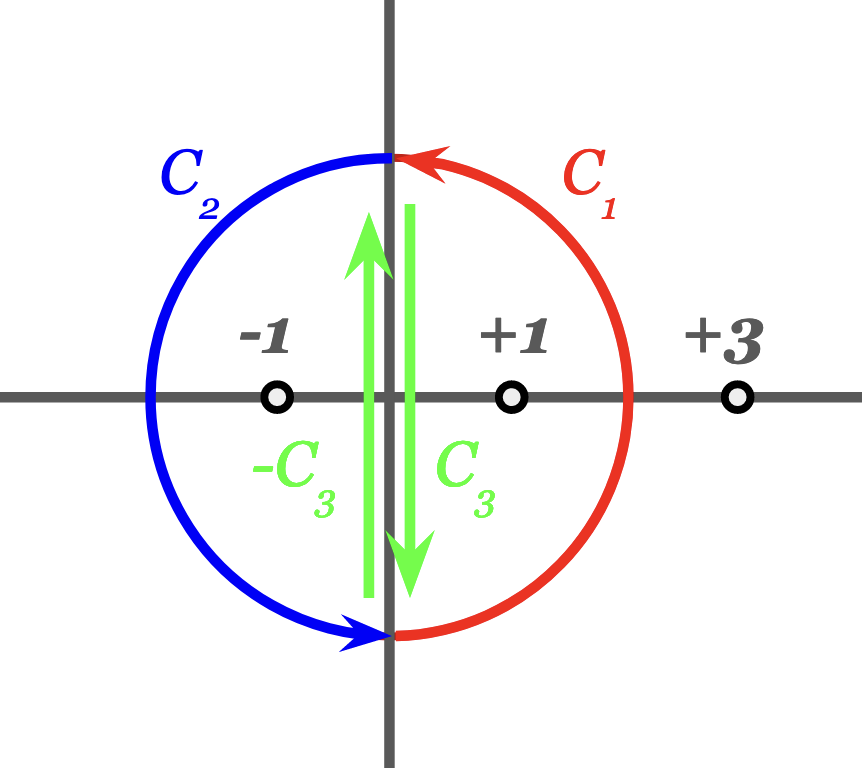
\includegraphics[width=0.5\textwidth]{images/hw_2/hw_2_2_5.png}
    \caption{\textcolor{red}{Червоним} відмічен контур $\mathcal{C}_1$, \textcolor{blue}{синім} контур $\mathcal{C}_2$, а \textcolor{green}{зеленим} відрізок $\mathcal{C}_3$ зверху-вниз}
    \label{fig:2_2_5}
\end{figure}

Тоді наш інтеграл запишемо як:
\[
\mathcal{I} = \int_{\mathcal{C}_1 + \mathcal{C}_3} \frac{dz}{(z-1)(z+1)(z-3)} + \int_{\mathcal{C}_2 - \mathcal{C}_3} \frac{dz}{(z-1)(z+1)(z-3)}
\]
Для першого інтеграла введемо $f(z) = \frac{1}{(z+1)(z-3)}$, а для другого $g(z) = \frac{1}{(z-1)(z-3)}$. Помітимо, що в такому разі $f$ є голоморфною у $\mathcal{C}_1 + \mathcal{C}_3$, а $g$ у $\mathcal{C}_2-\mathcal{C}_3$. В такому разі:
\[
\mathcal{I} = \int_{\mathcal{C}_1+\mathcal{C}_3} \frac{f(z)dz}{z-1} + \int_{\mathcal{C}_2-\mathcal{C}_3} \frac{g(z)dz}{z+1} = 2\pi i (f(1) + g(-1)) 
\]
Підставляємо значення:
\[
f(1) = \frac{1}{2 \cdot (-2)} = -\frac{1}{4}, \; g(-1) =\frac{1}{-2 \cdot (-4)} = \frac{1}{8}
\]
В такому разі:
\[
\mathcal{I} = 2\pi i \left(-\frac{1}{4} + \frac{1}{8}\right) = -\frac{\pi i}{4}
\]

\textbf{Відповідь.} $-\frac{\pi i}{4}$.

\end{document}

